\documentclass[a4j]{jarticle}
\usepackage[dvipdfmx]{graphicx}
\usepackage{here}
\usepackage{ascmac}
\usepackage{url}
\title{
\vspace{30mm}
株式会社マルナカ様\\
購入商品情報管理システム\\
外部設計書v1.0
\vspace{90mm}
}
\author{
株式会社Toron
}

\begin{document}
\maketitle
\newpage
\tableofcontents
\newpage

\section{ユーザインタフェース設計}


\subsubsection{管理者ログインページ}

図\ref{login}に管理者ページへのログインするためのページを示す。このページでは、ログインシステムの実装によって、管理者および各店舗の店長の判別を行うことができる。判別は、[ID]と[パスワード]によるベーシック認証によって行う。
\begin{figure}[H]
  \begin{center}
    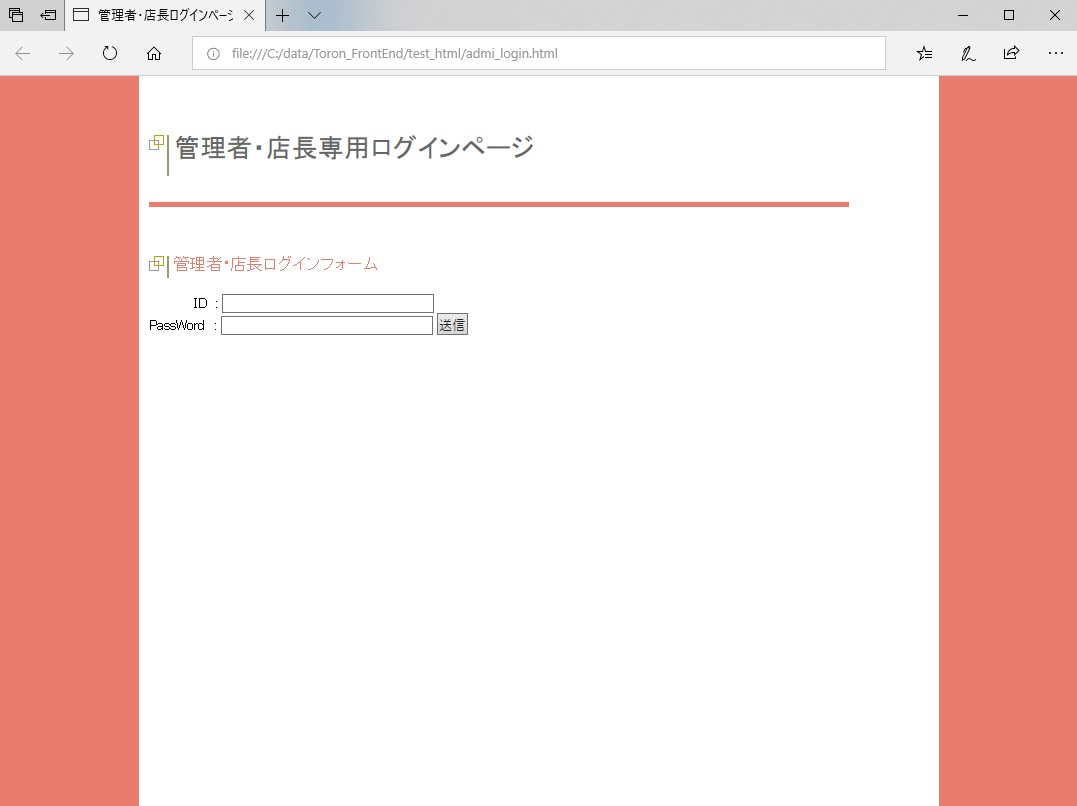
\includegraphics[width=15cm]{login.jpg} \\
    \caption{ログインページ}
    \label{login}
  \end{center}
\end{figure}

\begin{enumerate}
  \renewcommand{\labelenumi}{\textcircled{\scriptsize \theenumi}}
	\item 管理者・店長ログインフォーム\\
	管理者および店長が所持しているIDとパスワードを入力するフォームである。
	\item 送信ボタン\\
	ログインフォームに入力されたIDとパスワードを用いて、データベースにあるユーザーテーブルと照合を行う。IDやパスワードが入力されていなかったり、整合されるアカウントがない場合には、ログインエラーとし、図\ref{login2}のようなページが表示される。IDとパスワードが認証され、そのユーザーが管理者である場合、後述する管理者ページへ遷移する。そのユーザーが店長である場合、店長専用ページである特価情報管理ページへ遷移する。
\end{enumerate}
\begin{figure}[H]
  \begin{center}

    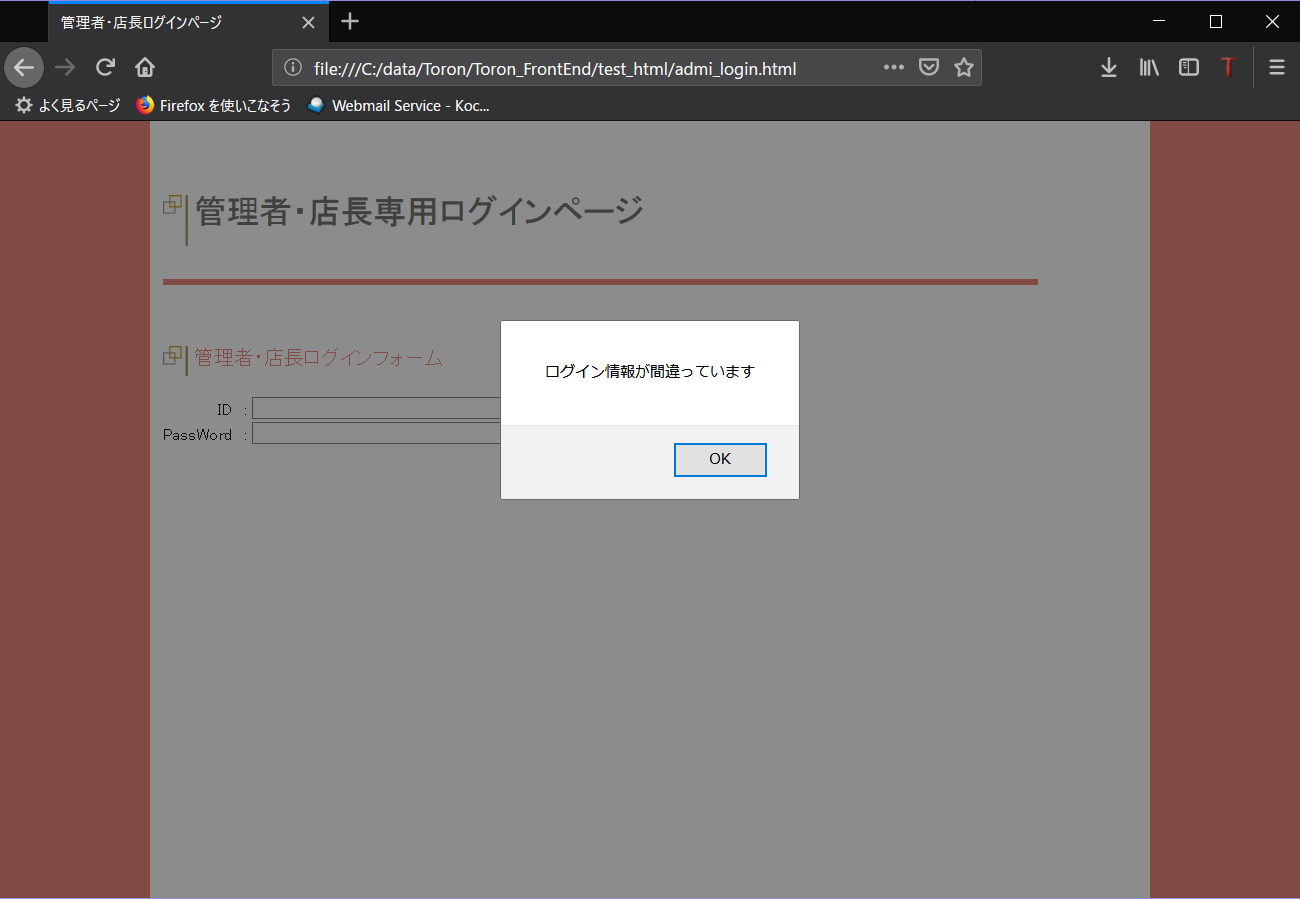
\includegraphics[width=15cm]{login2.png} \\
    \caption{ログイン失敗時の表示}
    \label{login2}
  \end{center}
\end{figure}

\subsubsection{管理者ページ}
図\ref{welcome1}にログイン後の管理者ページを示す.このページでは,店長管理ページと特売情報管理ページへ遷移することができる.
\begin{figure}[H]
  \begin{center}
    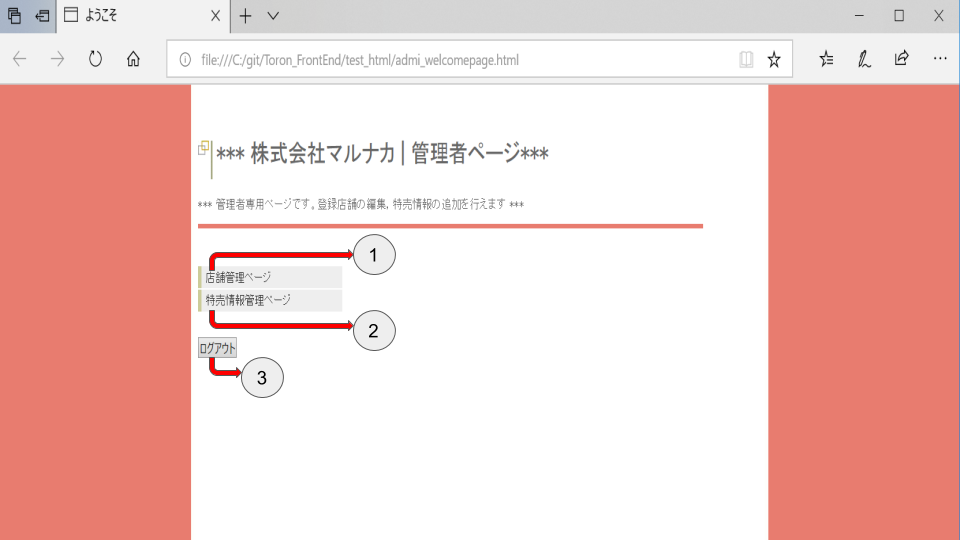
\includegraphics[width=15cm]{welcome1.png} \\
    \caption{管理者ページ}
    \label{welcome1}
  \end{center}
\end{figure}
\begin{enumerate}
  \renewcommand{\labelenumi}{\textcircled{\scriptsize \theenumi}}
	\item 店長管理ページボタン\\
	クリックすると,店長管理ページへ遷移する.
	\item 特売情報管理ページボタン\\
  クリックすると,特売情報管理ページへ遷移する.
\end{enumerate}

\subsubsection{店長管理ページ}
図\ref{tentyou1}に店長管理ページを示す.このページでは,マルナカ各店舗に所在する店長の管理を行うことができる.
\begin{figure}[H]
  \begin{center}
    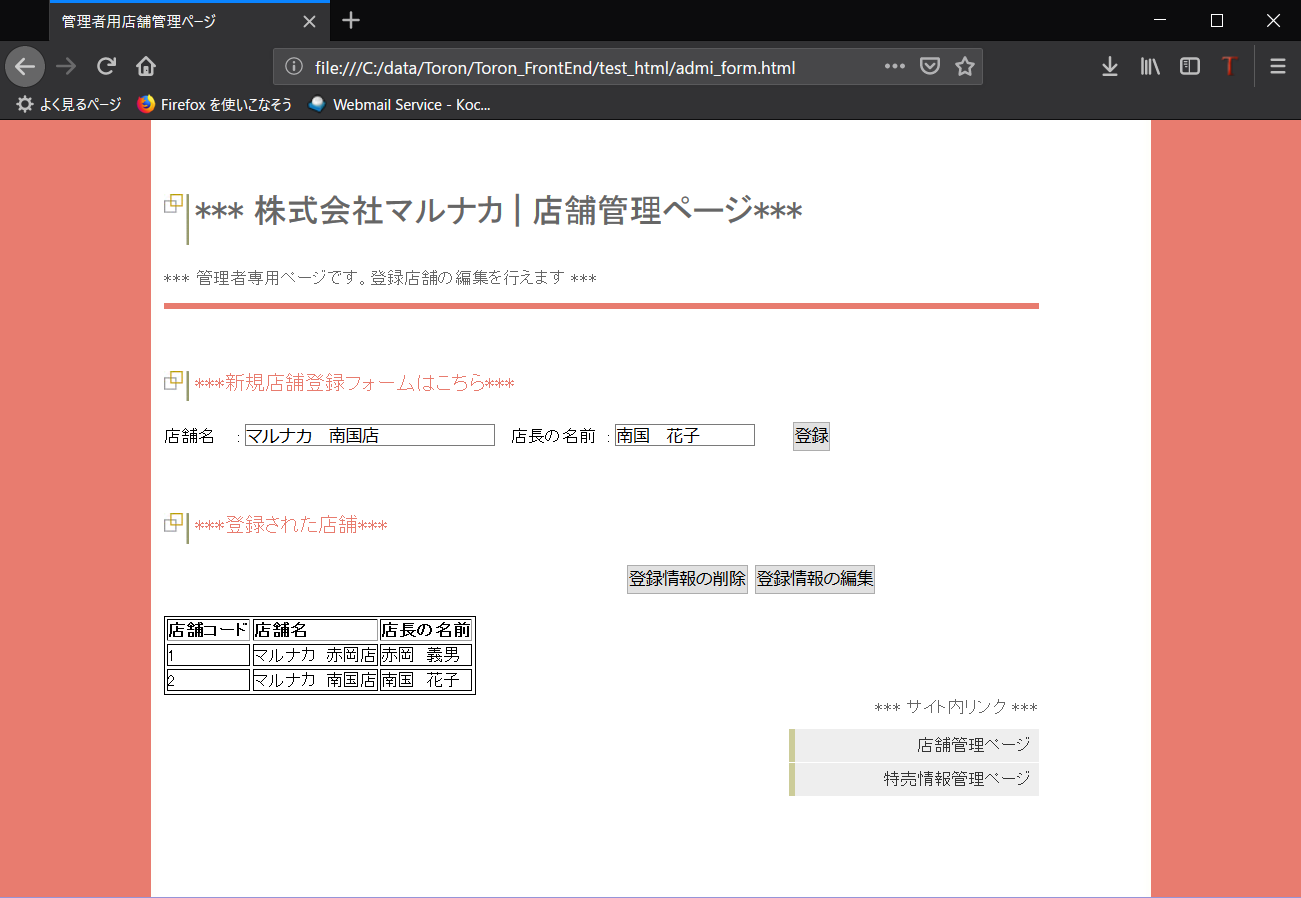
\includegraphics[width=15cm]{tentyou1.png}\\
    \caption{店長管理ページ}
    \label{tentyou1}
  \end{center}
\end{figure}



\begin{enumerate}
\renewcommand{\labelenumi}{\textcircled{\scriptsize \theenumi}}
\item 店舗名,名前入力フォーム\\
マルナカの配属される店舗と店長の名前を入力するフォームである.
\item 登録ボタン\\
入力フォームに入力された店舗名と店長名をデータベース上に書き込む.名前を元にユーザテーブルから参照し,その名前のユーザは自動的に権限が店長へと切り替わる.ユーザテーブルに該当する.ユーザが存在しない場合と店舗名が間違っている場合,既に登録されている場合には登録は行えない.
\item 登録情報更新ボタン\\

データベースに登録されている店舗情報と店長情報を更新する操作を行うことができるようになるボタンである。このボタンをクリックすると、テーブルの更新を直感的に行うことができる.その際にも,店舗名の重複,ユーザーが存在しない場合には更新は行えない.
\item 登録情報削除ボタン\\
店舗の閉店などで店舗情報が必要なくなった際には,店舗情報の削除をボタンから行うことができる.クリックすると,図\ref{tentyou2}のように店舗情報の表の横にボタンが出現し、そのボタンを押すことでデータベース上の店舗の削除を行える.

\item 特売商品の確認表\\

登録された店舗と店長の各報を閲覧することができる表である。上で記述したように、登録削除ボタンをクリックすると、各店舗情報の削除ボタンと編集終了ボタンが表中に現れる。

\item サイト内リンク\\

管理者ログインを行っている場合、ログアウトしなくとも店舗管理ページと特売情報管理ページの行き来ができるというリンク集である。
\begin{figure}[H]
  \begin{center}
    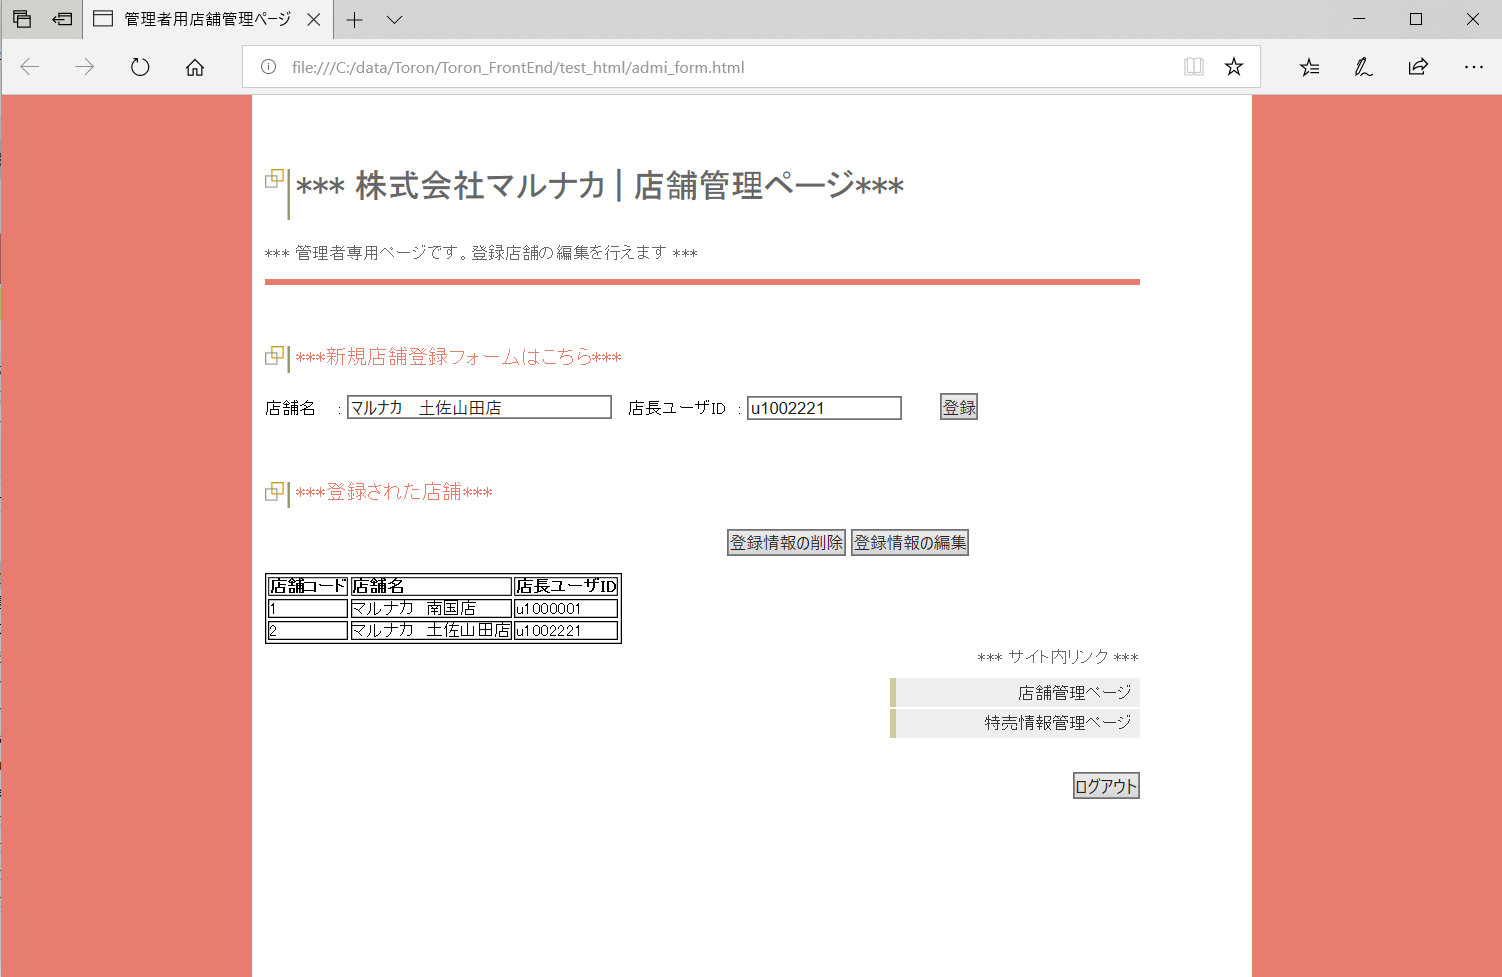
\includegraphics[width=15cm]{tentyou2.png}\\
    \caption{店舗情報削除時のページ表示}
    \label{tentyou2}
  \end{center}
\end{figure}
\end{enumerate}

\end{document}
